\clearpage
\newpage


\section{Segmentação Semântica}
\label{semantic}
No tocante às segmentações que fazem uso de técnicas de \textit{deep learning}, a segmentação semântica é uma das que fazem parte desse grupo, sendo que essas possuem o propósito de atribuir uma determinada classe, ou rótulo, para cada pixel presente em uma cena \citep{Wang2017, Ghosh2019, Shelhamer2016, Arbelaez2012,Zhang2018} o que é determinado como um trabalho de nível de pixel.

O uso de técnicas de segmentações semânticas tem sido útil para situações em que o contexto é desconhecido, visto que por meio dessas abordagens é possível entender à categoria dos objetos presentes na cena, assim como propriedades relacionadas a sua localização e os formatos dos objetos \citep{Zhang2018}, sendo de extrema importância para o trabalho com imagens médicas, sistemas autônomos e afins.

A saída de redes que pertencem à categoria de segmentação semântica comumente são uma máscara de 
pixels com uma única e determinada classe, o que pode ser visualizado na Figura \ref{semantic:fig:3}.

\begin{figure}[H]
   \caption{Segmentação semântica.}
   \centering
   \label{semantic:fig:3}
    \begin{subfigure}[t]{0.45\textwidth}
        \centering
        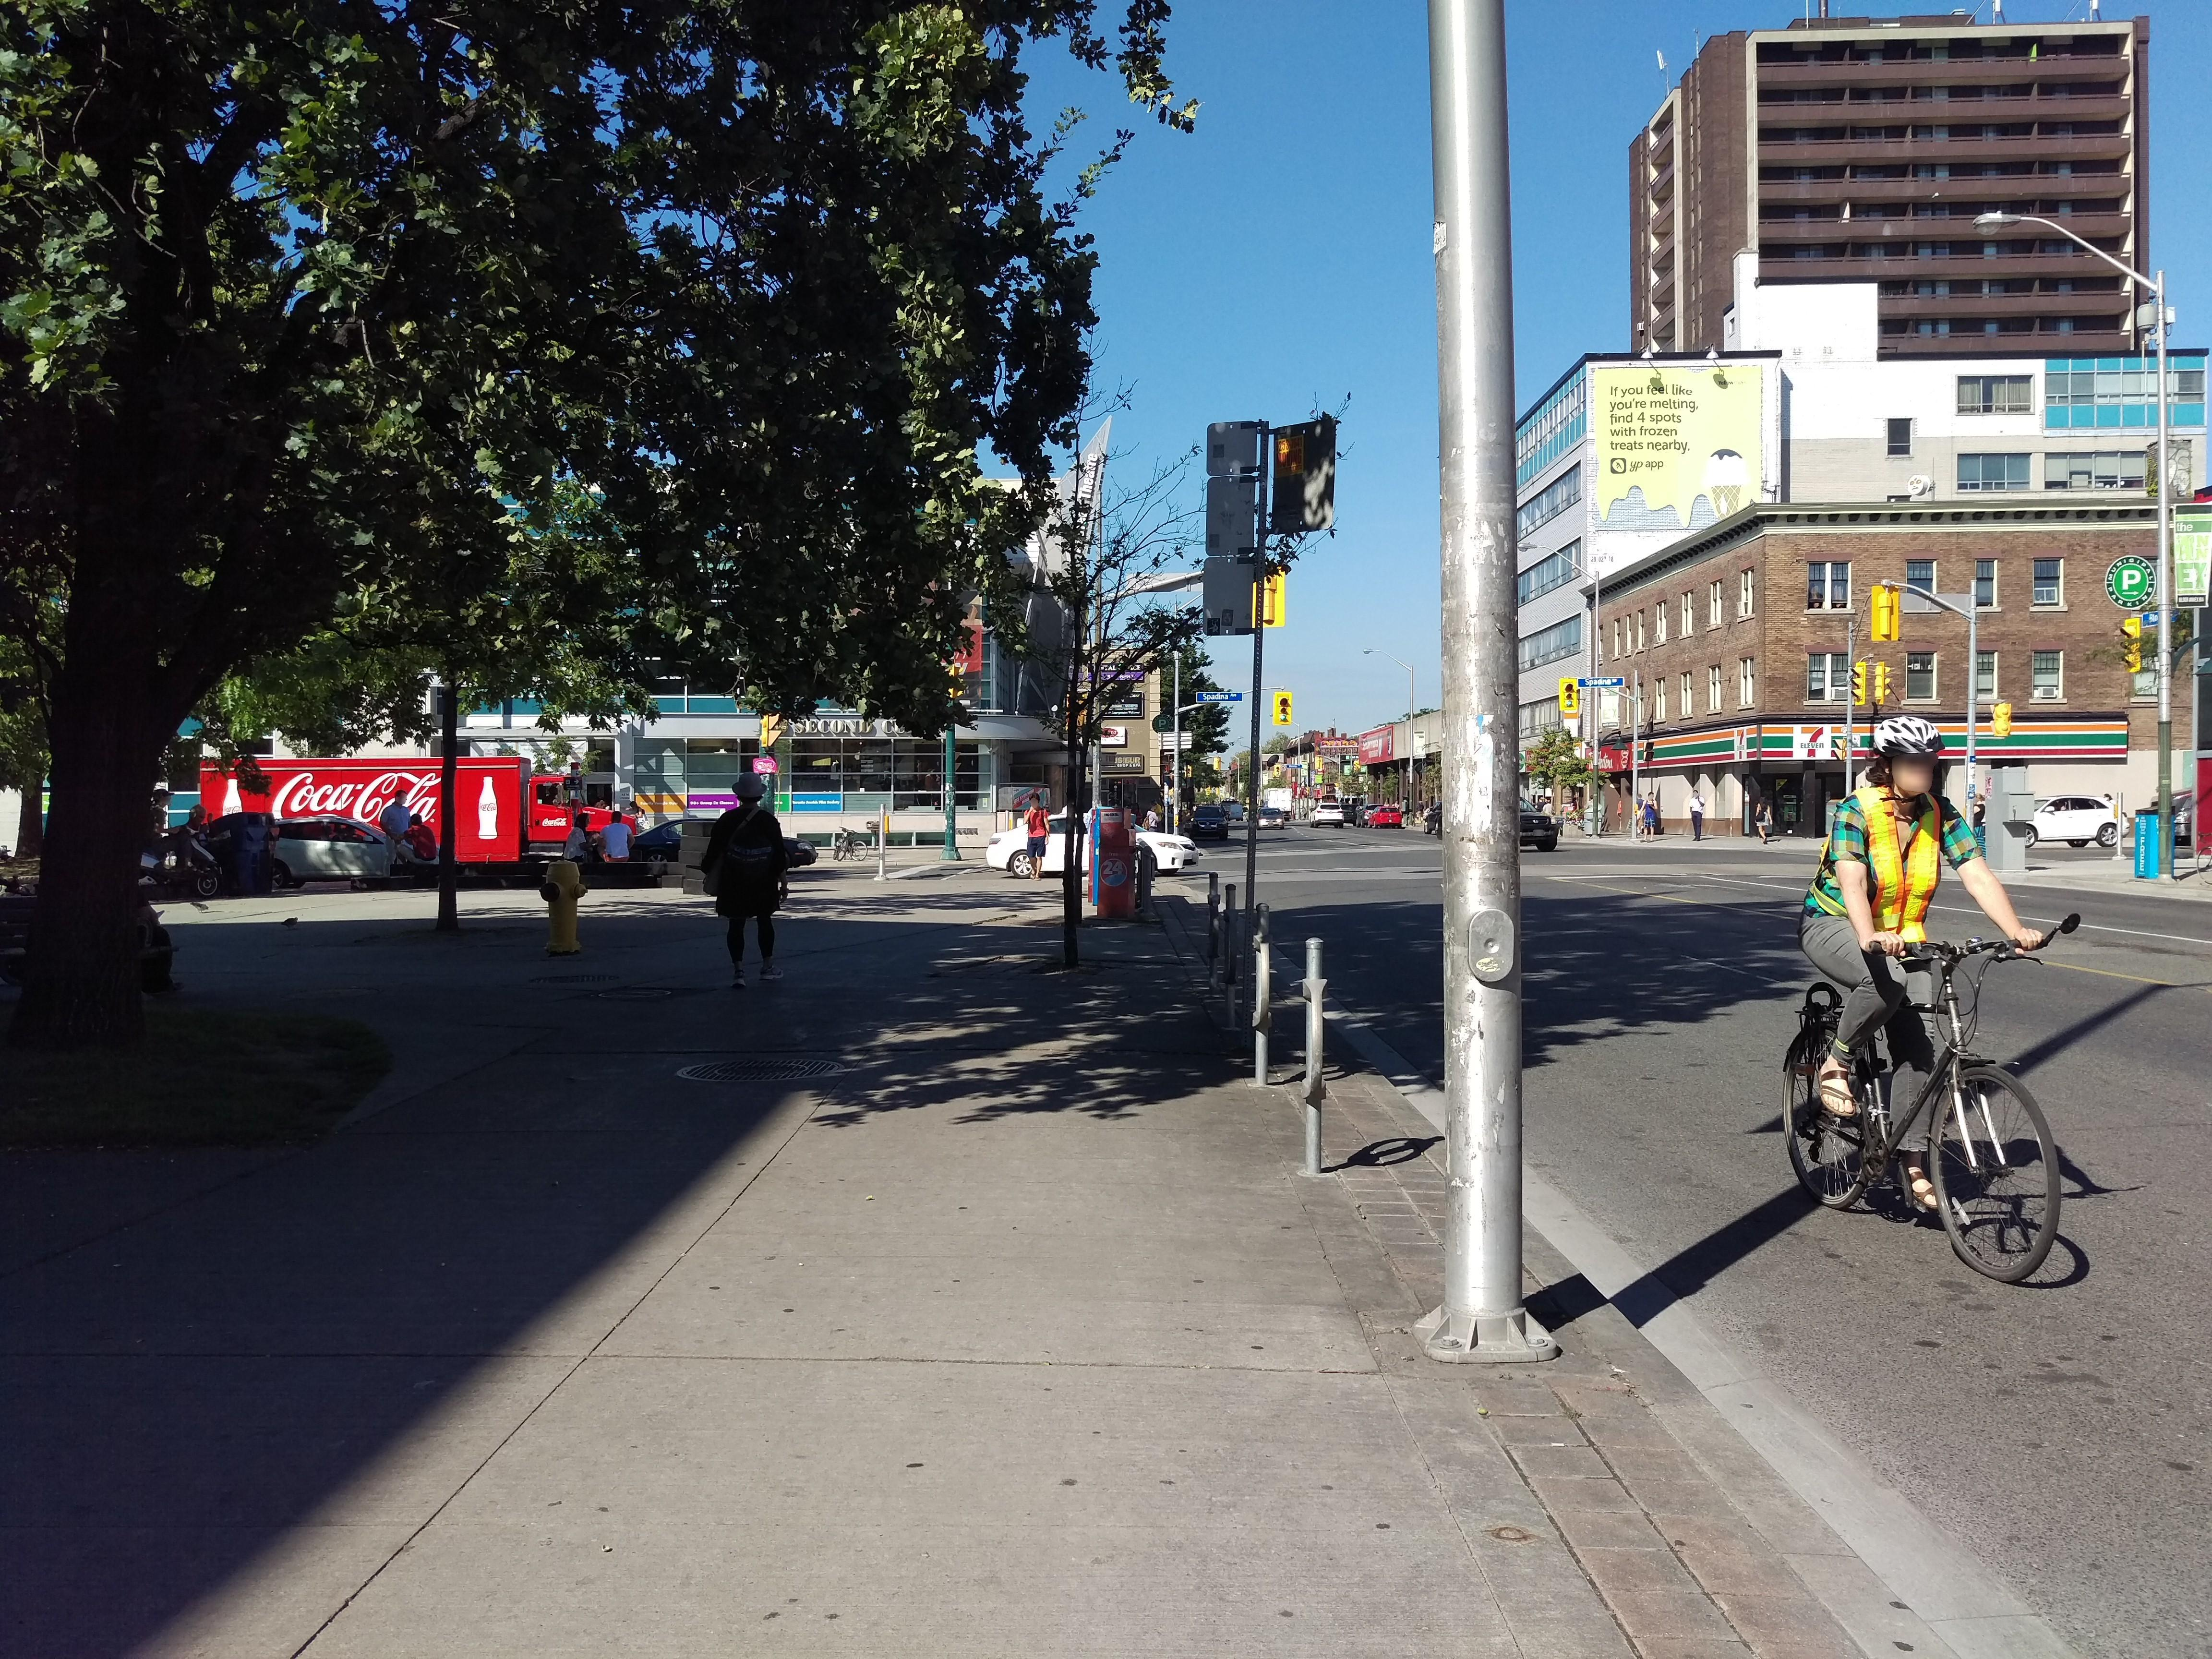
\includegraphics[height=1.5in]{recursos/imagens/semantic/t1.jpg}
        \caption{Imagem original.}
        \label{semantic:fig:3.1}
    \end{subfigure}%
    ~ 
    \begin{subfigure}[t]{0.45\textwidth}
        \centering
        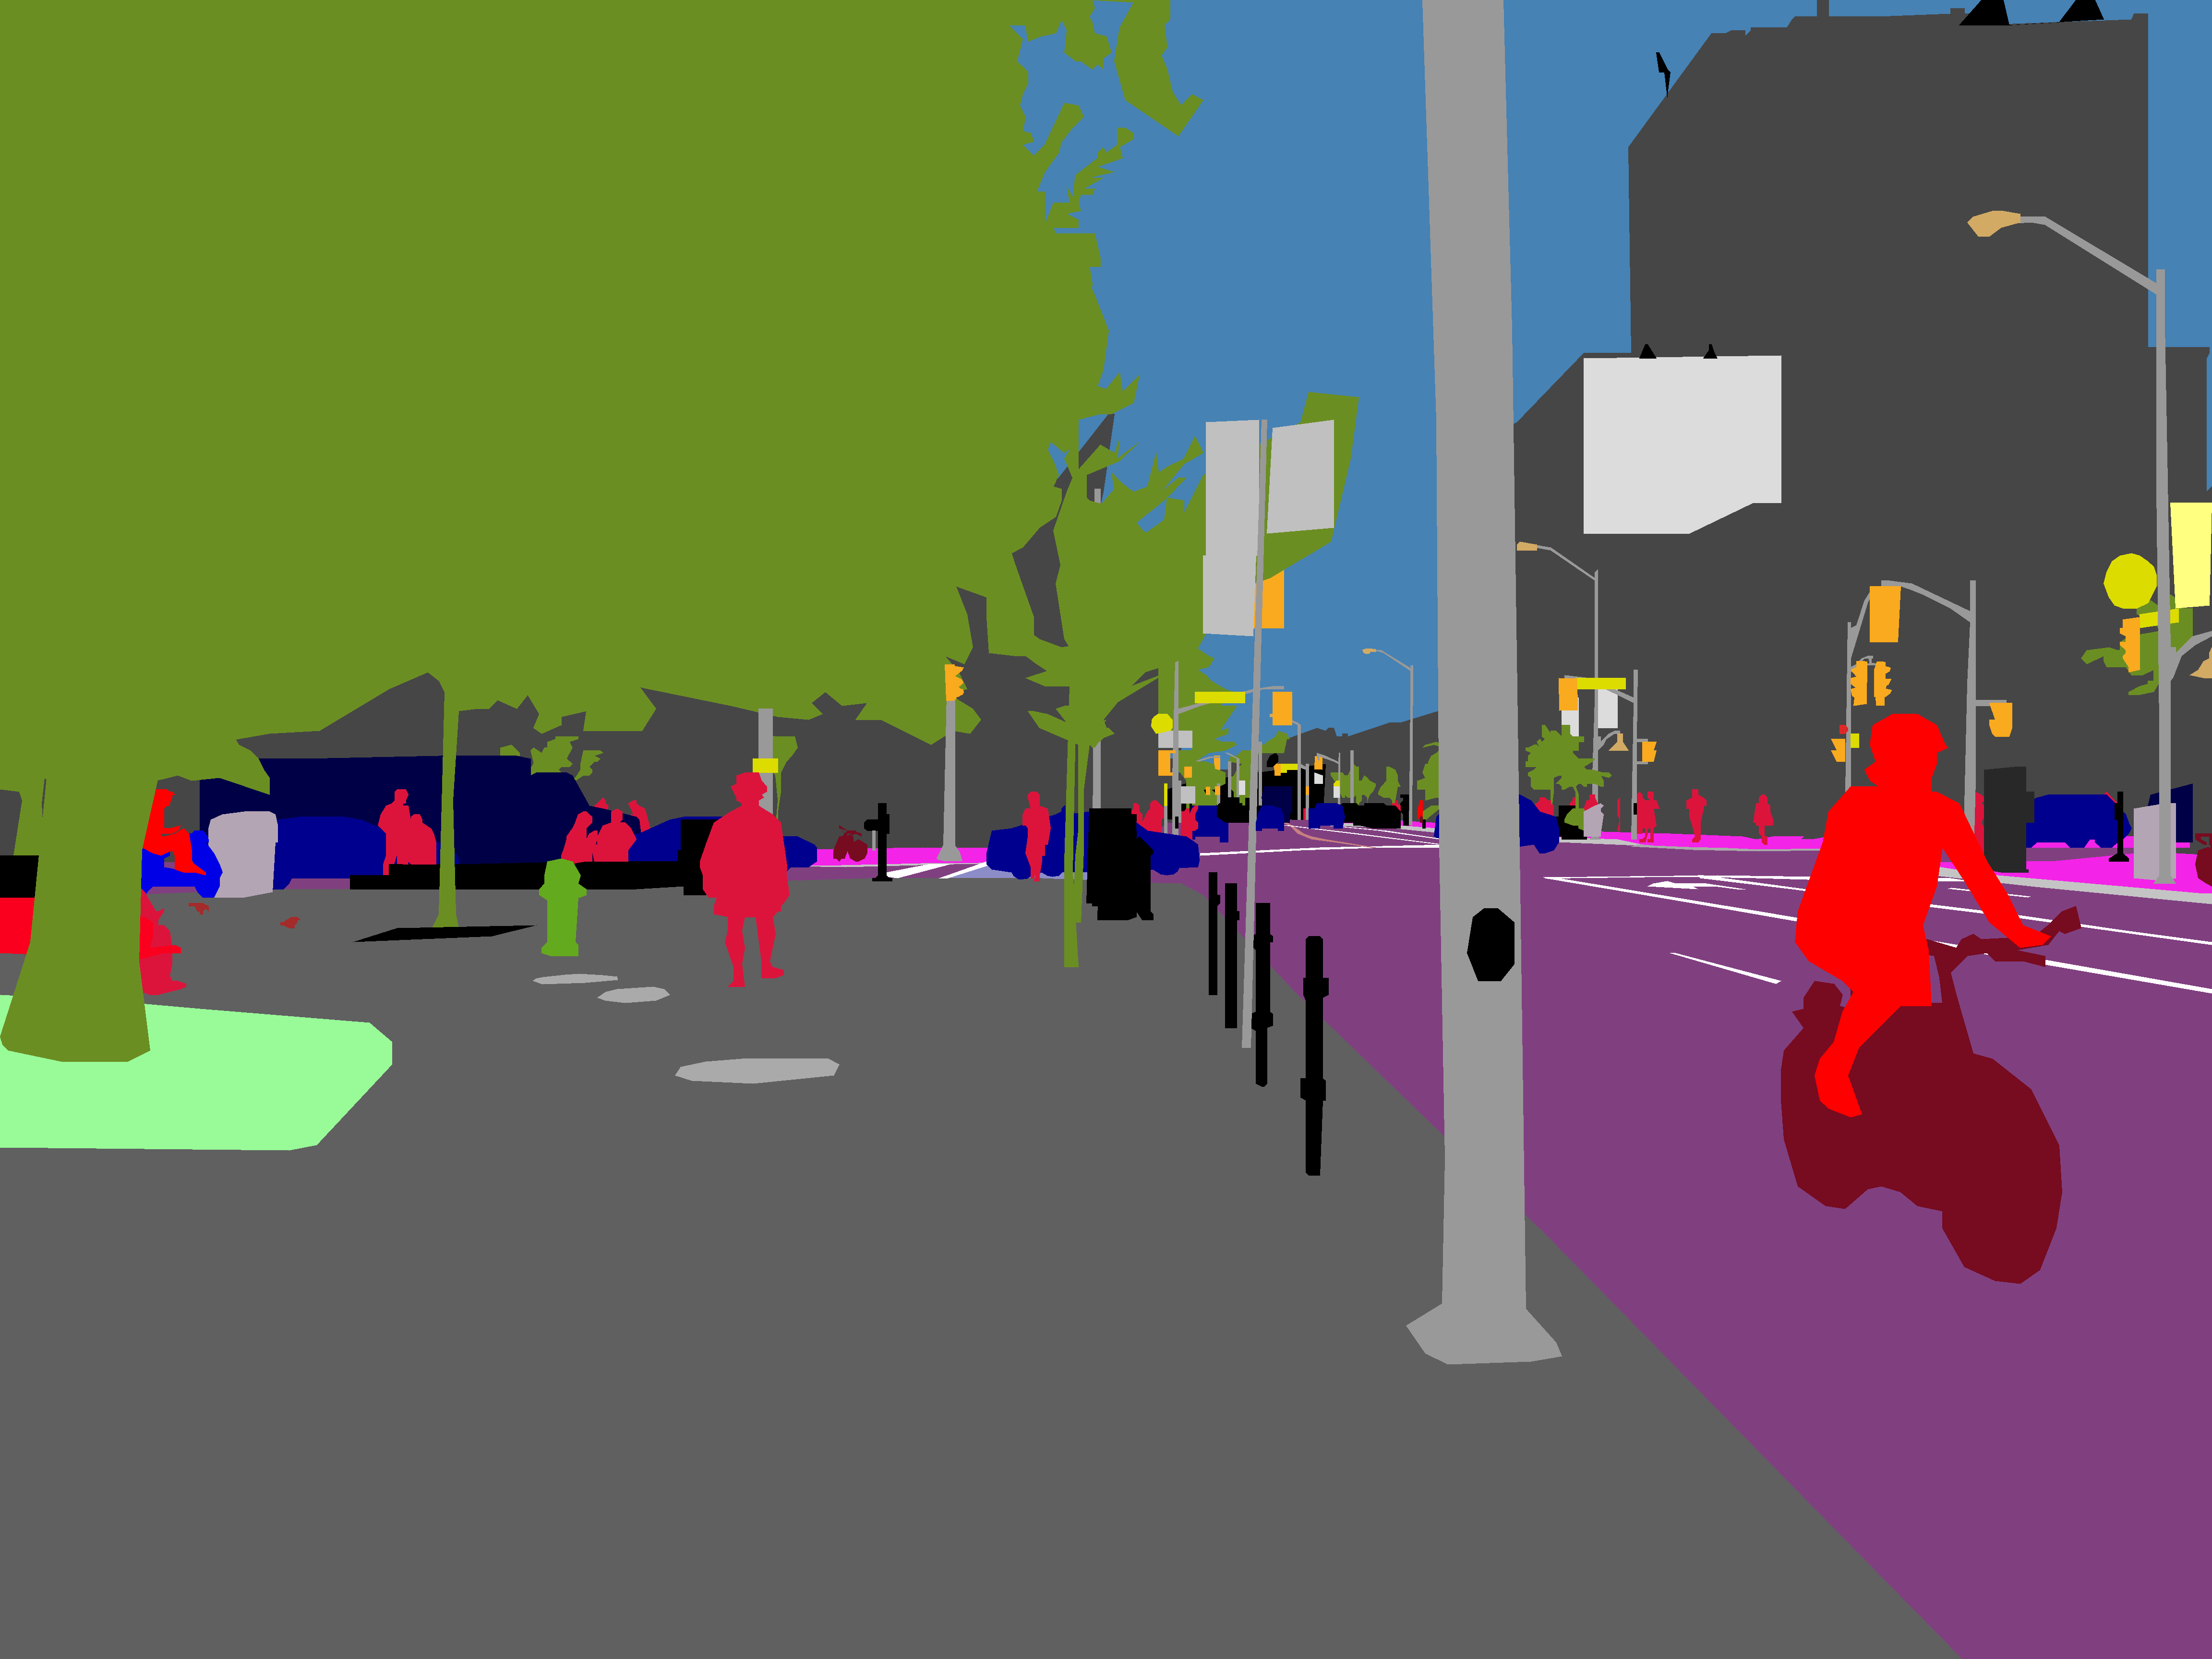
\includegraphics[height=1.5in]{recursos/imagens/semantic/s1.png}
        \caption{Segmentação semântica.}
        \label{semantic:fig:3.2}
    \end{subfigure}%

    Fonte: \cite{Neuhold2017_ICCV}.
\end{figure}

Sendo assim, neste capítulo, assuntos relacionados a abordagens de estado-da-arte nessa questão (Seção \ref{semantic:FCN}) e às métricas utilizadas para esse tipo de segmentação (Seção \ref{semantic:metrics}) serão detalhadamente trabalhados.


\subsection{Arquiteturas}
\label{semantic:arch}
Quando abordamos as arquiteturas para os modelos de segmentação semântica, é evidente o crescente desenvolvimento de oportunidades para resolver a problemática de separar classes de objetos a nível de pixel, como mencionado por \citep{Guo2018ANetworksb}. No contexto das arquiteturas de segmentação semântica, existe uma divisão relevante relacionada ao nível de supervisão da rede, que inclui abordagens totalmente supervisionadas, fracamente supervisionadas e semi-supervisionadas, conforme detalhado por \citep{Hao2020ALearning}. No entanto, este trabalho se concentra exclusivamente nas arquiteturas consideradas estado-da-arte na parte totalmente supervisionada, pressupondo a disponibilidade de dados de treinamento rotulados, incluindo imagens originais juntamente com suas respectivas máscaras anotadas \citep{Hao2020ALearning}.

Para esmiuçar mais sobre essas arquiteturas, é importante ressaltar a diferença em relação às CNNs convencionais, que tendem a perder detalhes espaciais devido aos processos de \textit{pooling} e convoluções. As redes de segmentação semântica, ao contrário, são mais atentas a esses detalhes. Nesse contexto, a colaboração adequada entre esses dois tipos de características possui o potencial de aprimorar significativamente o desempenho da segmentação semântica, seguindo a estratégia denominada de \quotes{aprimoramento de recursos}, a qual será explorada adiante.

\subsubsection{\textit{Fully Convolutional Networks} (FCN)}
\label{semantic:FCN}
Quando se trata de segmentações semânticas, várias arquiteturas e \textit{frameworks} são propostos para a resolução de problemas, de modo que garanta evolução quanto ao desempenho e às suas capacidades, contudo, o primeiro \textit{framework} a ser considerado estado-da-arte para esse atividade de segmentação baseia-se na arquitetura de \textit{Fully Convolutional Networks} \citep{Shelhamer2016} ou FCN, que propõem o trabalho apenas com camadas convolucionais - incluindo a última camada \citep{Hesamian2019}, como demonstrado na Figura \ref{semantic:fig:5} - assim, estabelecendo uma subamostragem de pixels (\textit{pixelwise}), seguida pela construção de um mapa de segmentação de mesmo tamanho que a imagem de entrada \citep{Minaee2021, Zhang2018, Hesamian2019}.

\begin{figure}[H]
    \centering
    \caption{Estrutura da arquitetura FCN.}
    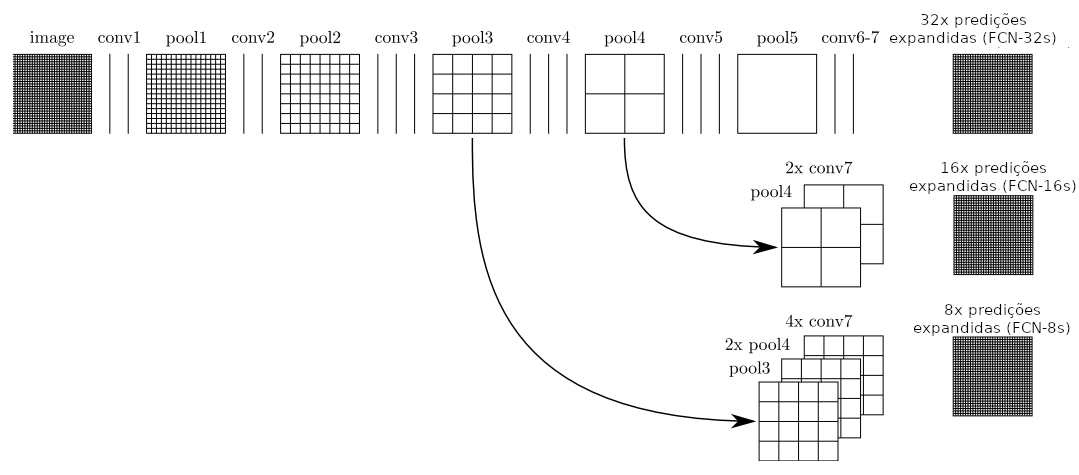
\includegraphics[width=1\linewidth]{recursos/imagens/semantic/fcn_arch.png}
    \label{semantic:fig:5}

    Fonte: retirada e adaptado de \cite{Shelhamer2016}.
\end{figure}

Essa configuração de FCN foi aplicada nos \textit{datasets} PASCAL VOC 2011 \citep{everingham2010pascal}, SIFT Flow \citep{Liu2011} e NYUDv2 \citep{Silberman:ECCV12} chegando a resultados de 90,3\% de PA e 62,7\% de \textit{mean IoU} no primeiro \textit{dataset} citado \citep{Ghosh2019} e estabelecendo referência de estado-da-arte em sua performance \citep{Minaee2021}.

Para sua configuração foram utilizados conceitos e modificações da arquitetura das CNNs VGG16 (explorada na Seção \ref{cnn:vgg}) e GoogLeNet \citep{Szegedy2015}, possibilitando a entrada e saída de tamanhos variados na rede \citep{Minaee2021}, de sorte que a entrada e saída tenham o mesmo tamanho, o que fica visível na Figura \ref{semantic:fig:6}.

\begin{figure}[H]
    \centering
    \caption{Representação de exemplo em FCN.}
    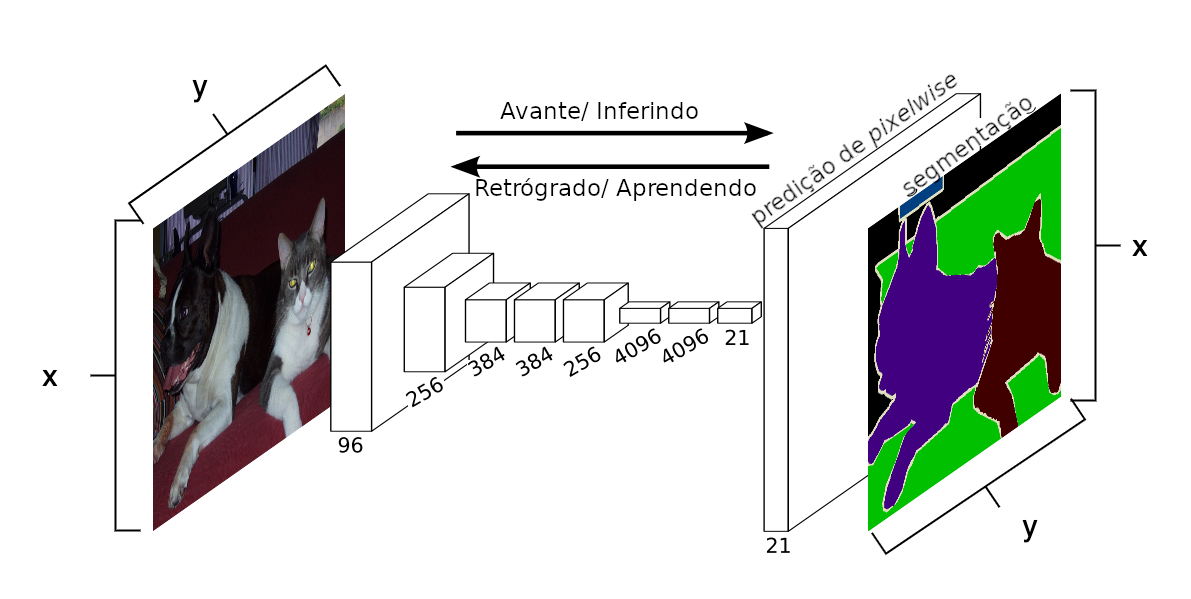
\includegraphics[width=1\linewidth]{recursos/imagens/semantic/fcn_example.png}
    \label{semantic:fig:6}

    Fonte: retirada e adaptado de \cite{Shelhamer2016}.
\end{figure}

Por fim, quanto às suas limitações, é informado que as configurações de FCN são ineficientes em trabalhos de segmentação 3D e para o uso em tempo real, visto que leva cerca de 100ms - em hardware não especificado pelo autor - para trabalhar com imagens de baixa resolução \citep{Minaee2021}, mas novas arquiteturas baseadas nesse modelo, como a ParseNet \citep{Liu2015} vêm evoluindo para suprir essas limitações.

\subsubsection{U-Net}
\label{semantic:unet}

No âmbito das arquiteturas voltadas para segmentação semântica, a evolução trouxe a U-Net \citep{Ronneberger2015U-net:Segmentation}, que se destacou após o período das FCNs. Introduzida em 2015, a U-Net rapidamente ganhou notoriedade, superando a popularidade das mencionadas FCNs \citep{Sultana2020EvolutionSurvey}.

As U-Nets operam com um caminho de contração (também conhecido como \textit{encoder}) que progressivamente reduz a resolução espacial dos dados e captura o contexto dos exemplos, seguido por um caminho de expansão simétrica (também conhecido como \textit{decoder}) que restaura a resolução original por meio de convoluções transpostas e realiza a segmentação. A estrutura se assemelha a um \quotes{U}, como retrata a Figura \ref{semantic:fig:unet}, o que levou à sugestão do nome da arquitetura. A conexão entre as camadas de \textit{encoder} e \textit{decoder}, conhecida como \quotes{\textit{skip connection}}, permite a preservação de informações de baixo nível e ajuda a mitigar problemas de perda de detalhes durante a redução da resolução \citep{Minaee2021, Minaee2021DeepClassification}. Por não conter camadas densas nas U-Nets, elas podem ser consideradas modelos baseados em FCNs \citep{Minaee2021}, sendo que a maior diferença entre essas arquiteturas está no uso de \quotes{\textit{skip connections}} entre as convoluções e \textit{up-samplings}, além da simetria das U-nets \citep{OZTURK2020ComparisonImageries}.

\begin{figure}[H]
    \centering
    \caption{Arquitetura U-Net.}
    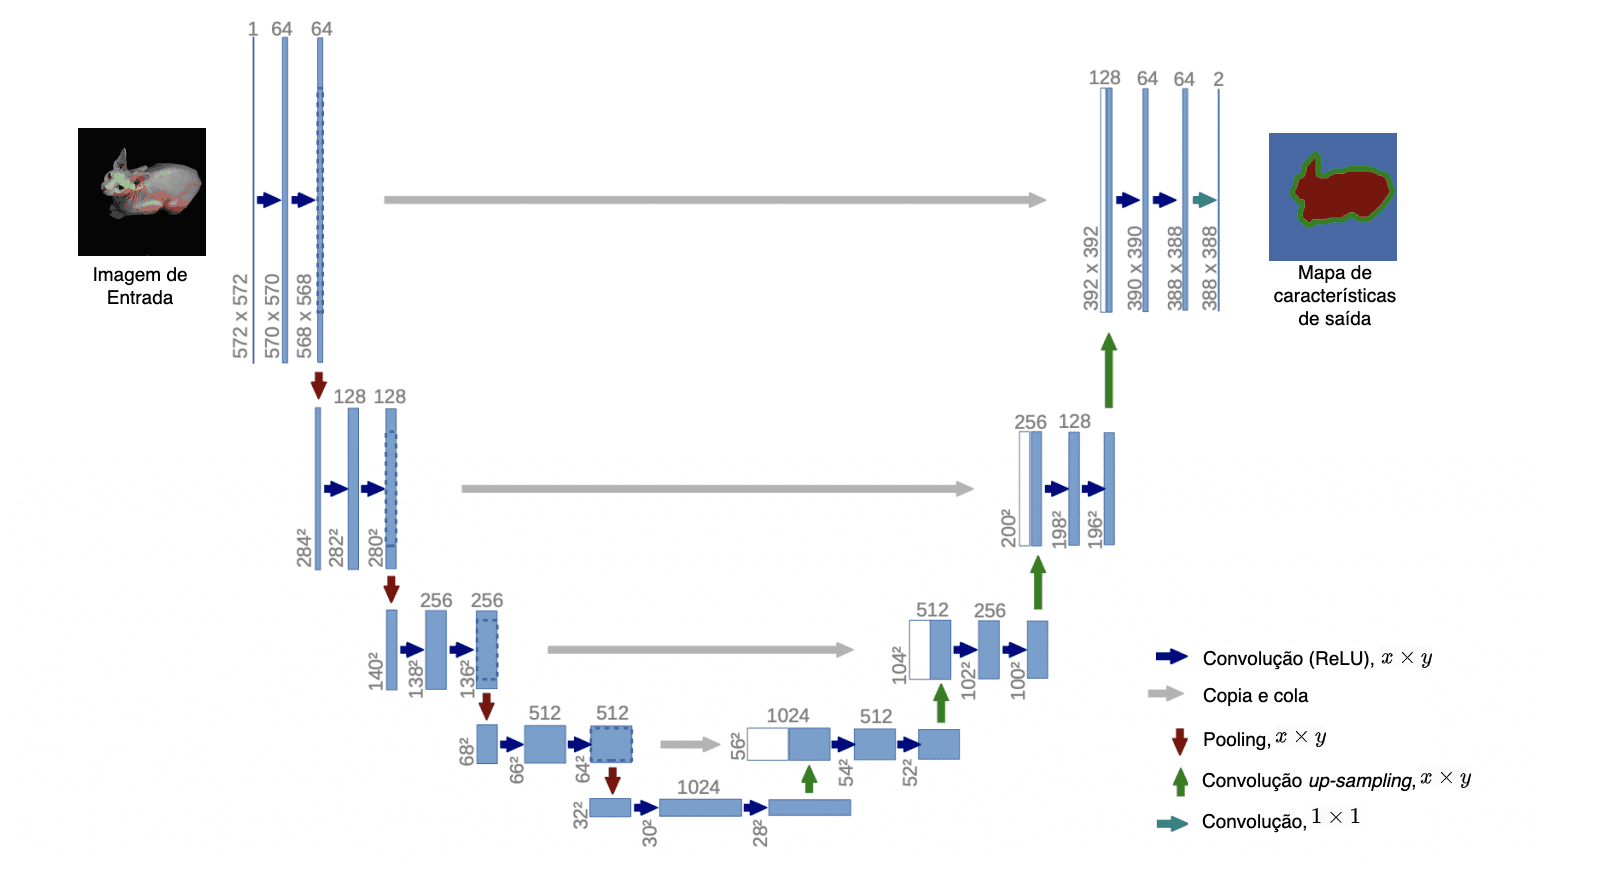
\includegraphics[width=1\linewidth]{recursos/imagens/semantic/unet-arch.png}
    \label{semantic:fig:unet}

    Fonte: retirada e adaptado de \cite{Ronneberger2015U-net:Segmentation}.
\end{figure}

As vantagens inerentes a essa arquitetura incluem uma capacidade robusta para lidar com imagens de tamanhos variados, permitindo a aplicação eficiente em diversos contextos, como na análise de imagens médicas \citep{Ronneberger2015U-net:Segmentation}. Além disso, as U-Nets têm a habilidade de aprender representações altamente significativas em diferentes níveis de abstração, o que as torna eficazes na captura de detalhes importantes em uma imagem \citep{Alom2019RecurrentSegmentation}. Também é importante destacar que essas redes têm a capacidade de reduzir a tendência de gerar segmentações excessivamente granulares, fornecendo segmentações mais suaves e coerentes \citep{Du2020MedicalReview}. No entanto, é fundamental reconhecer que, como qualquer abordagem, as U-Nets também possuem desvantagens. Em particular, essas redes frequentemente possuem um grande número de parâmetros, o que pode aumentar os requisitos computacionais e tornar o treinamento mais demorado, dependendo do tamanho do conjunto de dados e da complexidade da tarefa \citep{Ronneberger2015U-net:Segmentation}. Além disso, pela grande quantidade de convoluções, muitas vezes a informação espacial é perdida, segundo \cite{Zhang2023LcmUNet:Segmentation}.

Voltando ao contexto mais amplo, onde a segmentação semântica tem como objetivo atribuir rótulos de classe a cada pixel em uma imagem, a arquitetura da U-Net se mostra relevante e eficaz, sendo exemplificado pelos resultados obtidos desde seu desenvolvimento com \cite{Ronneberger2015U-net:Segmentation}. No entanto, questões que exploram a preservação da espacialidade da imagem durante a segmentação nesse tipo de estrutura ainda são pouco explorados, principalmente quando a proposta está em variações das tradicionais camadas de \textit{pooling} que são os atuais estado-da-arte \citep{Minaee2021}.

\subsubsection{U-Net-Like}


\subsection{Métricas}
\label{semantic:metrics}
Tendo dito que o objetivo principal das segmentações semânticas está relacionado com a assimilação de classes para cada um dos pixels presentes na imagem \cite{Csurka2013} fazem-se necessárias métricas que mensurem o desenvolvimento positivo ou negativo do modelo em questão.

Sendo assim, nesta seção, métricas comuns para a avaliação de segmentações semânticas serão discutidas: métricas baseadas em região (Sessão \ref{semantic:pa}), \textit{intersection over union} (Seção \ref{semantic:IoU}) e F1 \textit{Score} (Seção \ref{semantic:f1}).


\subsubsection{\textit{Pixel Accuracy}}
\label{semantic:pa}
A métrica de \textit{pixel accuracy} (PA) é uma das métricas mais simples utilizadas no contexto de segmentação semântica, em que, na prática, se resume na razão entre o pixel classificado corretamente em relação ao total de pixels na imagem \citep{Minaee2021}. Sendo assim, é possível expressar a sua fórmula pela Equação \ref{semantic:eq:1}:

\begin{equation}
    \label{semantic:eq:1}
    PA = \frac{\sum_{i=0}^{K} p_{ij}}{\sum_{i=0}^{K} \sum_{j=0}^{K} p_{ij}},
\end{equation}
sendo $K$ as classes presentes na imagem, independente se para um plano de fundo ou para primeiro plano, e $p_{ij}$ é o número de pixels preditos como ($i$) pertencentes à classe $j$.

Todavia, é relevante citar que essa métrica indicando apenas precisão dos pixels, como o nome sugere, não é adequada para situações que há um desequilíbrio de classes, situação em que determinadas classes dominam a cena e que se faz presente no mundo real.


\subsubsection{\textit{Intersection over Union} (IoU)}
\label{semantic:IoU}
Já a métrica de intersecção entre a união, do inglês \textit{Intersection over Union} (IoU) ou Jaccard Index, é uma métrica que não passa por problemas de desbalanceamento de classes, além de ser considerada uma das métricas mais comuns para esse tipo de atividade \cite{Minaee2021}.

Sua representação pode ser visualizada a partir da Figura \ref{semantic:fig:1}, além de que pela Equação \ref{semantic:eq:2} é possível entender que o resultado de IoU se dá pela razão entre a intersecção da segmentação predita (A) e \textit{ground truth} (B), e a união entre a segmentação predita e o \textit{ground truth}, ou seja,

\begin{equation}
    \label{semantic:eq:2}
    IoU = J(A,B) = \frac{|A \cap B|}{|A \cup B|}.
\end{equation}

\begin{figure}[H]
    \centering
    \caption{Representação de IoU.}
    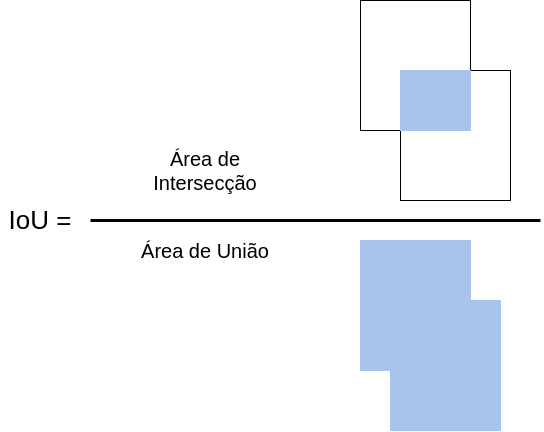
\includegraphics[height=2.3in]{recursos/imagens/semantic/IoU.png}
    \label{semantic:fig:1}

    Fonte: do próprio autor.
\end{figure}

\subsubsection{\textit{Mean Intersection Over Union} (MIoU)}
\begin{sloppypar}
Após a criação dessa métrica, outras variações ganharam repercussão, das quais destaca-se \textit{Mean Intersection-over-Union (mIoU)}, a qual realiza a média entre todos os valores de IoU das classes presentes na cena e apresenta um valor escalar como resultado para a segmentação como um todo \cite{Minaee2021}, sendo utilizada em trabalhos como \cite{Mohan2020}.
\end{sloppypar}


\subsubsection{F1 \textit{Score}}
\label{semantic:f1}
Para a definição da métrica F1-\textit{score}, que é extremamente comum na esfera de segmentação de imagens, é necessário ter ciência de antemão que ela é composta pelo uso de outras duas métricas, sendo elas: 1) precisão, que é a divisão de verdadeiros positivos pela soma de verdadeiros positivos e falsos positivos; 2) revocação, que é a divisão de verdadeiros positivos pela soma de verdadeiros positivos e falsos negativos, como mostrados nas Equações \ref{semantic:eq:3} e \ref{semantic:eq:4}, respectivamente,

\begin{equation}
    \label{semantic:eq:3}
    \text{Precisão} = \frac{VP}{VP + FP}
\end{equation}
e
\begin{equation}
    \label{semantic:eq:4}
    \text{Revocação} = \frac{VP}{VP + FN}.
\end{equation}

Assim, para a definição de F1-\textit{score} é utilizada a média harmônica entre a precisão e revocação \cite{Minaee2021}, a qual pode ser expressa pela Equação \ref{semantic:eq:5}:

\begin{equation}
    \label{semantic:eq:5}
    F1-score = \frac{2 . \text{Precisão} . \text{Revocação}}{\text{Precisão} + \text{Revocação}}.
\end{equation}

Por fim, vale comentar que para situações em que tem-se uma segmentação binária, o valor de F1-\textit{score} é semelhante ao valor do coeficiente Dice, o qual normalmente é utilizado para situações médicas \cite{Minaee2021} e utiliza conceitos de intersecção assim como a métrica de IoU (Seção \ref{semantic:IoU}), visto que quando não está assimilado a situações binárias, pode ser representado pela Equação \ref{semantic:eq:6} ou pela Figura \ref{semantic:fig:2}:

\begin{equation}
    \label{semantic:eq:6}
    Dice = \frac{2|A \cap B|}{|A| + |B|}.
\end{equation}

\begin{figure}[H]
    \centering
    \caption{Representação do coeficiente Dice.}
    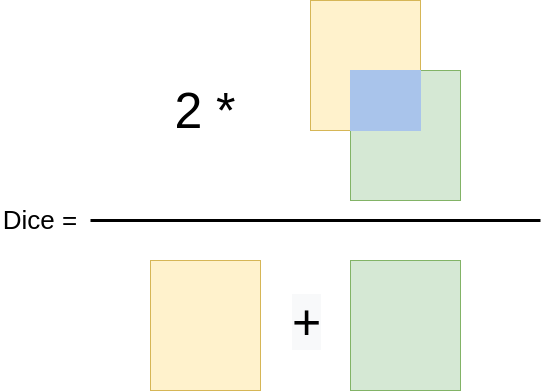
\includegraphics[height=2.3in]{recursos/imagens/semantic/dice.png}
    \label{semantic:fig:2}

    Fonte: do próprio autor.
\end{figure}

\subsection{Considerações Finais do Capítulo}
\label{semantic:conclusion}
Concluindo em relação a segmentações semânticas, pode-se dizer que são um grande avanço quando comparadas a tarefas de detecção de objetos, como ocorre em \cite{Vaillant1994}, visto que esse novo modelo de segmentações possibilita o trabalho com mais dados em relação às cenas, como citado neste capitulo (Capítulo \ref{semantic}).

Entretanto, essa rede possui dificuldade quando o problema em questão está relacionado à separação de objetos que possuem a mesma classe, mas são objetos diferentes, visto que não há uma separação por indivíduos \cite{Kirillov2019a} como é possível observar na Figura \ref{semantic:fig:4.1}, em que todas as pessoas próximas se encontram conectadas ou em situações que se torna necessária a segmentação minuciosa de uma cena \cite{Ghosh2019}, como as partes do corpo de uma pessoa, por exemplo.

\begin{figure}[H]
   \caption{Exemplo de segmentação semântica com instâncias unificadas.}
   \centering
   \label{semantic:fig:4}
    \begin{subfigure}[t]{0.6\textwidth}
        \centering
        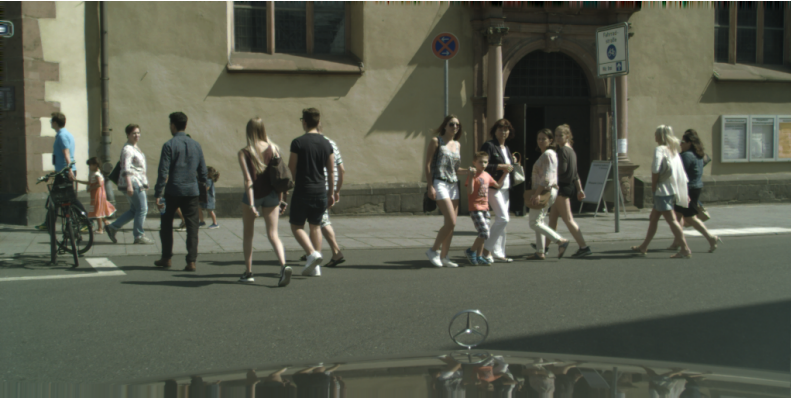
\includegraphics[width=1\linewidth]{recursos/imagens/semantic/sema_ori.png}
        \caption{Imagem original.}
        \label{semantic:fig:4.1}
    \end{subfigure}%
    ~ 

    \begin{subfigure}[t]{0.6\textwidth}
        \centering
        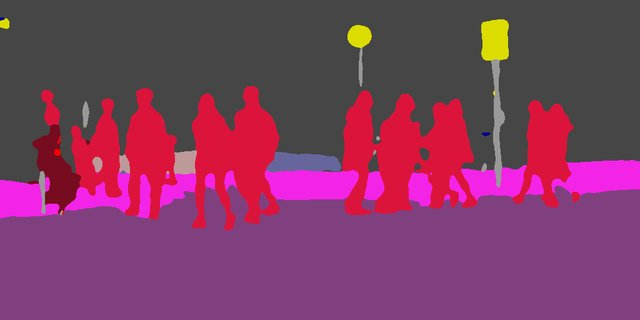
\includegraphics[width=1\linewidth]{recursos/imagens/semantic/sema_unified.png}
        \caption{Segmentação com instâncias unificadas.}
        \label{semantic:fig:4.2}
    \end{subfigure}%

    Fonte: \cite{Fischer2017}.
\end{figure}

Por fim, vale destacar que modelos de segmentação semântica não são recomendados para sistemas que precisam realizar segmentações próximas de um tempo real, levando em conta câmeras com menos de 25 quadros por segundo, devido ao seu desempenho, como aponta \cite{Minaee2021}.